\documentclass{article}

\usepackage{indentfirst}
\usepackage{graphicx}
\usepackage{listings}
\usepackage{fancyhdr}
\usepackage{hyperref}
\usepackage{amsmath}
\usepackage{amssymb}

\title{CIC0097 - Banco de Dados: Projeto \\
        \large \textbf{Tema:} Rede Social}
\author{Guilherme da Rocha Cunha - 221030007 \\
        \and
        Arthur Diehl Barroso - 221029991 \\
        \and
        Eduardo Quirino de Oliveira - 211010305 \\
        \and 
        Breno Costa Avelino Lima - 211010280}
\date{2024.1}

\begin{document}

\pagestyle{fancy}

\maketitle

\begin{figure}[ht]
        \centering
        
\includegraphics[width=.5\textwidth]{imagens/logo_unb.jpg}
\end{figure}

\newpage

\fancyhead{}
\fancyfoot[C]{\thepage}


\renewcommand*\contentsname{Sumário}
\tableofcontents

\newpage

\section{Introdução}
O projeto consiste na aplicação dos conhecimentos adquiridos na disciplina "CIC0097 - Banco de Dados". O banco de dados construído, com o tema Rede Social, utilizou como mecanismo de armazenamento o SQLite e o programa com as funções CRUD foi-se implementado na linguagem Python utilizando o framework web Flask.

\section{Diagrama de Entidade Relacionamento}
O diagrama abaixo representa o modelo entidade relacionamento do projeto.

\begin{figure}[!ht]
        \centering
        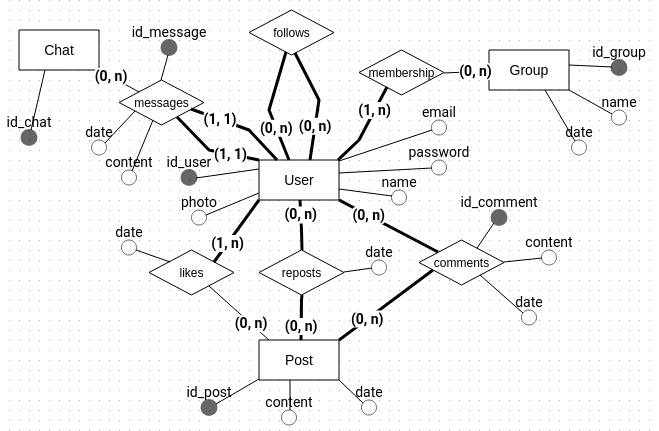
\includegraphics[width=1\textwidth]{imagens/mer.png}
        \caption{Modelo Entidade Relacional}
\end{figure}

\subsection{Entidades}
\subsubsection{User}
\paragraph{Definição:} Representa um usuário no sistema.
\begin{itemize}
        \item Atributo chave: \verb|id_user|.
        \item Atributos simples: \verb|email|, \verb|password|, \verb|name| e \verb|photo|.
\end{itemize}

\subsubsection{Post}
\paragraph{Definição:} Uma publicação feita por um usuário.
\begin{itemize}
        \item Atributo chave: \verb|id_post|.
        \item Atributos simples: \verb|content| e \verb|date|.
\end{itemize}

\subsubsection{Group}
\paragraph{Definição:} Um grupo composto de usuários, similar à grupos do Facebook, comunidades do Orkut e dentre outros.
\begin{itemize}
        \item Atributo chave: \verb|id_group|.
        \item Atributos simples: \verb|name| e \verb|content|.
\end{itemize}

\subsubsection{Chat}
\paragraph{Definição:} Local de conversa entre dois usuários.
\begin{itemize}
        \item Atributo chave: \verb|id_chat|.
\end{itemize}

\subsection{Relacionamentos}
As entidades se relacionam de 6 maneiras distintas:
\begin{enumerate}
        \item Likes: um usuário pode curtir $n$ publicações e uma publicação pode ser curtida por $n$ usuários. Post tem participação total na relação, isto é, toda publicação é feita por algum usuário, mas nem todo usuário faz uma publicação (participação parcial).
        \item Reposts: um usuário pode repostar $n$ publicações e uma publicação pode ser repostada por $n$ usuários. Ambas as entidades têm participação parcial no diagrama.
        \item Comments: um usuário pode fazer $n$ comentários em uma publicação e uma publicação pode ter $n$ usuários comentando.
\end{enumerate}

\section{Modelo Relacional}

\begin{figure}[!ht]
        \centering
        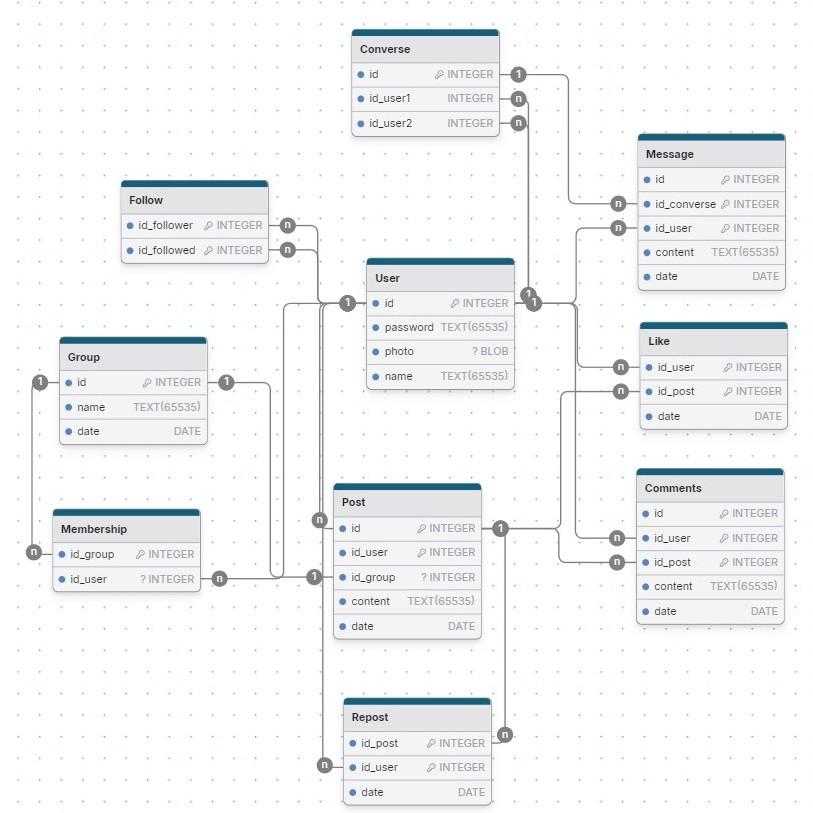
\includegraphics[width=1\textwidth]{imagens/mr.jpg}
        \caption{Modelo Relacional}
\end{figure}

\section{Consultas em Álgebra Relacional}

\section{Avaliação das formas normais}

\section{Diagrama da Camada de Mapeamento}

\section{Referências}
\begin{itemize}
        \item ELMASRI, R., NAVATHE, S. B., Sistemas de Banco de Dados, Sétima Edição, 2019, Editora Addison Wesley.
        \item HEUSER, C. A. , Projeto de banco de Dados, Editora Sagra Luzzatto
        \item Ferramenta de Modelagem MER: \href{https://app.brmodeloweb.com/#!/conceptual/66dd8939bb821248818df271}{app.brmodeloweb.com}
        \item Ferramenta de Modelagem MR: \href{https://drawdb.vercel.app/}{drawdb.verce.app}
\end{itemize}

Repositório do projeto: \href{https://github.com/qrno/BD-2024-1}{link}.

\end{document}